\chapter{Testing}
\label{chap:testing} 

Dieses Kapitel beschreibt wie wir unseren Bot und dessen Komponenten getestet haben. Das Testen beanspruchte ein grosser Teil unserer aufgewendeten Zeit. Die nachfolgenden Methoden zeigen auf wie wir versuchten m�glichst effizient zu testen, so dass uns mehr Zeit f�r das implementieren von Modulen blieb. Es stellte sich heraus, dass das Implementieren und Testen von neuem Code in UnitTests, anstatt direkt im Bot, zeitsparender war und weniger M�he bereitete Fehler zu finden. 

\section{UnitTests}
\label{sec:testCenter.UnitTests}

Dank dem modularen Aufbau des Java-Codes war es uns m�glich einzelne Module zu testen. F�r unsere UnitTests verwendeten wir die JUnit 4 Library. So findet man in jedem Java Project das Code-Package und ein UnitTest-Package, welches den Code auf dessen Richtigkeit pr�ft. Die Module erst nach den erfolgreichen UnitTests in den Bot eingebaut. Dies hat den Vorteil, dass die Fehlern nicht im laufenden Spiel auftraten und wir die Ursachen  m�hsam suchen mussten.\\
Um das Modul CombatPositioning\footnote{siehe im Code unter Startegy.tactics.combat} zu realisieren haben wir sogar 'Test Driven Development' eingesetzt. Dass heisst, wir haben zuerst den Test mit Ausgangslage, Aufruf von CombatPositioning, und das erwartete Resultat als UnitTest geschrieben. Danach wurde solange an CombatPositioning programmiert, bis das erwartete Testresultat eintraf.

\section{Visuelle Tests}
\label{sec:testCenter.VisuelleTests}

In Form eines UnitTest haben wir auch unsere visuellen Tests geschrieben. Eine visuelle �berpr�fung des Resultats ist meistens, vor allem bei der Pfadsuche, einfacher zu kontrollieren. Im Gegensatz zu JUnit wo das zu erwartende Resultat mit der Methode \texttt{assertEquals()} gepr�ft wird, haben die visuellen Test ein HTML-File als Output. In das HTML-File wird die Karte in Tabellenform gespeichert. In jeder Zelle der Tabelle k�nnen Objekte (Einheiten, H�gel, Wegpunkte etc.) durch farbige Punkte dargestellt werden. Diese Funktionalit�ten bietet die extra daf�r geschriebene Klasse MapOutput. Nachfolgend ist ein HTML-File abgebildet mit welchem wir die Korrektheit des Clustering und des HPA* Algorithmus visuelle �berpr�ft haben. 

\begin{figure}[H]
\centering
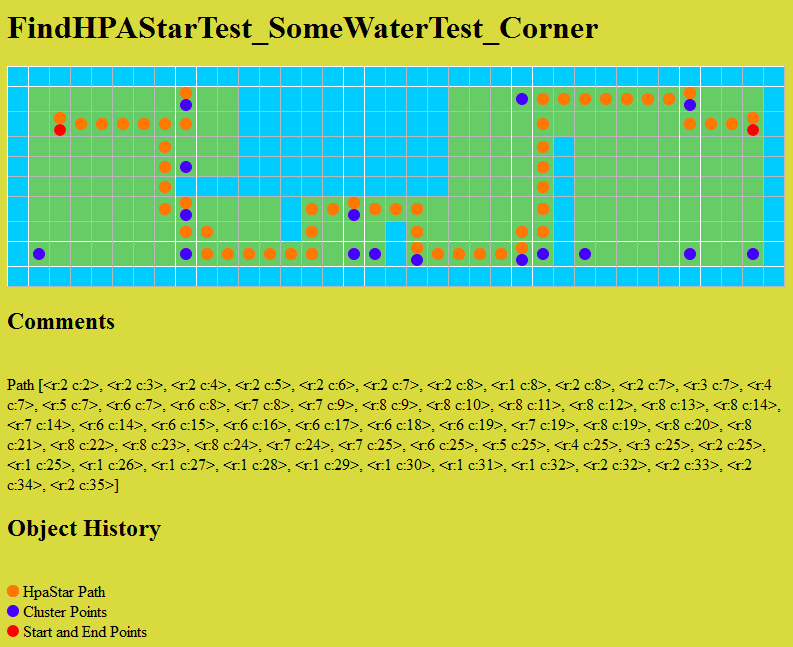
\includegraphics[height=100mm]{91_bilder/mapoutput01}
\caption{HTML-Ausgabe zur visuellen �berpr�fung von HPA*}
\label{fig:mapoutput01}
\end{figure}